\documentclass[journal,12pt,twocolumn]{IEEEtran}

\usepackage{setspace}
\usepackage{gensymb}
\singlespacing
\usepackage[cmex10]{amsmath}

\usepackage{amsthm}

\usepackage{mathrsfs}
\usepackage{txfonts}
\usepackage{stfloats}
\usepackage{bm}
\usepackage{cite}
\usepackage{cases}
\usepackage{subfig}

\usepackage{longtable}
\usepackage{multirow}

\usepackage{enumitem}
\usepackage{mathtools}
\usepackage{steinmetz}
\usepackage{tikz}
\usepackage{circuitikz}
\usepackage{verbatim}
\usepackage{tfrupee}
\usepackage[breaklinks=true]{hyperref}
\usepackage{graphicx}
\usepackage{tkz-euclide}


\usetikzlibrary{calc,math}
\usepackage{listings}
    \usepackage{color}                                            %%
    \usepackage{array}                                            %%
    \usepackage{longtable}                                        %%
    \usepackage{calc}                                             %%
    \usepackage{multirow}                                         %%
    \usepackage{hhline}                                           %%
    \usepackage{ifthen}                                           %%
    \usepackage{lscape}     
\usepackage{multicol}
\usepackage{chngcntr}

\DeclareMathOperator*{\Res}{Res}

\renewcommand\thesection{\arabic{section}}
\renewcommand\thesubsection{\thesection.\arabic{subsection}}
\renewcommand\thesubsubsection{\thesubsection.\arabic{subsubsection}}

\renewcommand\thesectiondis{\arabic{section}}
\renewcommand\thesubsectiondis{\thesectiondis.\arabic{subsection}}
\renewcommand\thesubsubsectiondis{\thesubsectiondis.\arabic{subsubsection}}



\hyphenation{op-tical net-works semi-conduc-tor}
\def\inputGnumericTable{}                                 %%

\lstset{
%language=C,
frame=single, 
breaklines=true,
columns=fullflexible
}
\begin{document}


\newtheorem{theorem}{Theorem}[section]
\newtheorem{problem}{Problem}
\newtheorem{proposition}{Proposition}[section]
\newtheorem{lemma}{Lemma}[section]
\newtheorem{corollary}[theorem]{Corollary}
\newtheorem{example}{Example}[section]
\newtheorem{definition}[problem]{Definition}

\newcommand{\BEQA}{\begin{eqnarray}}
\newcommand{\EEQA}{\end{eqnarray}}
\newcommand{\define}{\stackrel{\triangle}{=}}
\bibliographystyle{IEEEtran}
\raggedbottom
\setlength{\parindent}{0pt}
\providecommand{\mbf}{\mathbf}
\providecommand{\pr}[1]{\ensuremath{\Pr\left(#1\right)}}
\providecommand{\qfunc}[1]{\ensuremath{Q\left(#1\right)}}
\providecommand{\sbrak}[1]{\ensuremath{{}\left[#1\right]}}
\providecommand{\lsbrak}[1]{\ensuremath{{}\left[#1\right.}}
\providecommand{\rsbrak}[1]{\ensuremath{{}\left.#1\right]}}
\providecommand{\brak}[1]{\ensuremath{\left(#1\right)}}
\providecommand{\lbrak}[1]{\ensuremath{\left(#1\right.}}
\providecommand{\rbrak}[1]{\ensuremath{\left.#1\right)}}
\providecommand{\cbrak}[1]{\ensuremath{\left\{#1\right\}}}
\providecommand{\lcbrak}[1]{\ensuremath{\left\{#1\right.}}
\providecommand{\rcbrak}[1]{\ensuremath{\left.#1\right\}}}
\theoremstyle{remark}
\newtheorem{rem}{Remark}
\newcommand{\sgn}{\mathop{\mathrm{sgn}}}
\providecommand{\abs}[1]{\vert#1\vert}
\providecommand{\res}[1]{\Res\displaylimits_{#1}} 
\providecommand{\norm}[1]{\lVert#1\rVert}
%\providecommand{\norm}[1]{\lVert#1\rVert}
\providecommand{\mtx}[1]{\mathbf{#1}}
\providecommand{\mean}[1]{E[ #1 ]}
\providecommand{\fourier}{\overset{\mathcal{F}}{ \rightleftharpoons}}
%\providecommand{\hilbert}{\overset{\mathcal{H}}{ \rightleftharpoons}}
\providecommand{\system}{\overset{\mathcal{H}}{ \longleftrightarrow}}
	%\newcommand{\solution}[2]{\textbf{Solution:}{#1}}
\newcommand{\solution}{\noindent \textbf{Solution: }}
\newcommand{\cosec}{\,\text{cosec}\,}
\providecommand{\dec}[2]{\ensuremath{\overset{#1}{\underset{#2}{\gtrless}}}}
\newcommand*{\permcomb}[4][0mu]{{{}^{#3}\mkern#1#2_{#4}}}
\newcommand*{\perm}[1][-3mu]{\permcomb[#1]{P}}
\newcommand*{\comb}[1][-1mu]{\permcomb[#1]{C}}
\newcommand{\myvec}[1]{\ensuremath{\begin{pmatrix}#1\end{pmatrix}}}
\newcommand{\mydet}[1]{\ensuremath{\begin{vmatrix}#1\end{vmatrix}}}
\numberwithin{equation}{subsection}
\makeatletter
\@addtoreset{figure}{problem}
\makeatother
\let\StandardTheFigure\thefigure
\let\vec\mathbf
\renewcommand{\thefigure}{\theproblem}
\def\putbox#1#2#3{\makebox[0in][l]{\makebox[#1][l]{}\raisebox{\baselineskip}[0in][0in]{\raisebox{#2}[0in][0in]{#3}}}}
     \def\rightbox#1{\makebox[0in][r]{#1}}
     \def\centbox#1{\makebox[0in]{#1}}
     \def\topbox#1{\raisebox{-\baselineskip}[0in][0in]{#1}}
     \def\midbox#1{\raisebox{-0.5\baselineskip}[0in][0in]{#1}}
\vspace{3cm}
\title{Assignment 4}
\author{Raghav Juyal - EP20BTECH11018}
\maketitle
\newpage
\bigskip
\renewcommand{\thefigure}{\theenumi}
\renewcommand{\thetable}{\theenumi}
Download all python codes from 
\begin{lstlisting}
https://github.com/RaghavJuyal/AI1103/blob/main/Assignment4/Codes/Assignment4.py
\end{lstlisting}
%
and latex-tikz codes from 
%
\begin{lstlisting}
https://github.com/RaghavJuyal/AI1103/tree/main/Assignment4/Assignment4.tex
\end{lstlisting}
\section*{Question 15, GATE CS 2018}
Two people, P and Q decide to independently roll two identical dice, each with 6 faces, numbered 1 to 6. The person with the lower number wins. In case of a tie, they roll the dice repeatedly until there is no tie. Define a trial as a throw of the dice by P and Q. Assume that all 6 numbers on each dice are equi-probable and that all trials are independent. The probability that one of them wins on the third trial is?
\section*{Solution}
Let $p$ represent probability of a tie and $q$ represent probability that one of them wins. 
\begin{align}
    p &= 1\times\frac{1}{6} = \frac{1}{6}\\
    q &= 1-p = \frac{5}{6}
\end{align}
\vspace{-5mm}
\begin{figure}[h]
    \centering
     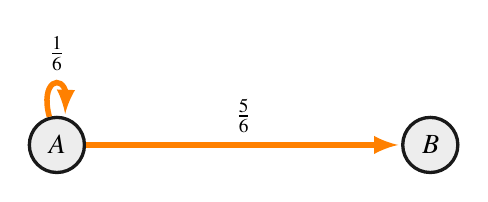
\begin{tikzpicture}[
roundnode/.style={circle, draw=black!90, fill=black!7, very thick, minimum size=7mm},
]
%Nodes
\node[roundnode]        (Tie)        {$A$};
\node[roundnode]        (owin)       [right=4cm of Tie] {$B$};
%Lines
 \draw[every loop,
        auto=right,
        line width=0.7mm,
        >=latex,
        draw=orange,
        fill=orange]
            (Tie) edge[ auto=left]  node {$\frac{5}{6}$} (owin)
            (Tie) edge[loop above]             node {$\frac{1}{6}$} (Tie);
\end{tikzpicture}
    \par{Markov Diagram where $A$ represents a tie and $B$ represents that one of P and Q wins}
\end{figure}\vspace{3mm}\\
The state transition matrix $P$ is shown below :
\begin{align*}
\begin{array}{c c} &
\begin{array}{c c} A  & B \\
\end{array}
\\
\begin{array}{c c}
A \\[3pt]
B
\end{array}
&
\left[
\begin{array}{c c}
\frac{1}{6} & 0 \\[2pt]
\frac{5}{6} & 0 \\
\end{array}
\right]
\end{array}
\end{align*}
Here the initial state, representing the first roll, $S_0$ is:\\
\begin{align*}
    S_0 = 
    \left[
\begin{array}{c}
\frac{1}{6} \\[3pt]
\frac{5}{6} \\
\end{array}
\right]
\end{align*}
For the $n^{th}$ state we have
\begin{align}
    S_n = P^n\times S_0
\end{align}
To get a win on the third trial we need the $(2,1)^{th}$ position of $S_2$.
\begin{align}
    S_2 &= P^2\times S_0 \nonumber\\
    &= \left[
\begin{array}{c}
\frac{1}{216} \\[2pt]
\frac{5}{216} \\
\end{array}
\right]
\end{align}
$\therefore$ The required probability is $\frac{5}{216}$

\end{document}